\documentclass[10pt]{article}
\usepackage{icmlko}

\icmlmeta{IP 파운데이션 월드모델}{240}{겹말}{판을 올린 ``새 축''은 이미 판에 있었다 --- 정보가 0 인 복사본이 같은 값을 낸다}

\begin{document}

\twocolumn[
\icmlheader

\begin{abstract}
노트 239가 웹툰 레코드에서 \textbf{태그 수}를 찾아 판을 $+$0.0038 올렸다. 이번에
그 절차 --- 학습 구간 연도 통제 상관 $\times$ 시간 다섯 조각 부호 일치 --- 를 여섯
도메인으로 넓혔다. 여섯이 다 통과했고, 넷을 넣으니 판이 0.4546에서
\textbf{0.4420으로 내려앉았다}($t{=}-2.71$). 갈랐다. 이름 공유가 아니고(공유
0.4420 대 분리 0.4412), 분포 이동이 아니고(KS 로 재면 제일 크게 흔들린 축이 제일
많이 \emph{돕는} 축이다), 지표 열 중복이 아니다(빼도 $-$0.0270 $\to$ $-$0.0269).
범인은 \textbf{모바일 price 하나}였다($-$0.0270, $t{=}-5.76$). 그런데 price 는
\textbf{그 열을 보지도 못하는 웹툰}을 0.4080에서 0.3380으로 무너뜨린다 --- 공유
계수를 빼앗아서다(\texttt{entry\_friction} 계수가 56\% 깎인다). 소스를 열어
보니 \texttt{entry\_friction} $=$ \texttt{scale01(price, 0, 15)} 이고
\texttt{target\_breadth} $=$ \texttt{scale01(n\_tag, 3, 14)} 다. \textbf{내가 찾은
``새 축''은 이미 판에 있던 축이다}(순위 상관 웹툰 $+$0.985 · 세계애니 · 만화 ·
애니 $+$1.000 · 모바일 $-$0.959). 그러면 이득은 어디서 왔나. \textbf{있는 열을
그대로 복사해서 넣어 봤다 --- $+$0.0100($t{=}2.70$)}, 새 열의 $+$0.0106과 같다.
정보가 0 인 열이 같은 값을 낸다. 이득은 자료가 아니라 \textbf{그 방향의 능형
벌점이 절반이 된 것}이고, 전역 alpha 를 $20{\to}10$ 으로 내리는 것으로는 재현이
안 된다($-$0.0001) --- 축 하나에만 걸리는 가중이라서다. \textbf{노트 239와 이번
노트의 이득을 둘 다 취소한다.} 판은 0.4584에서 \textbf{0.4546으로 내린다.}
가드 열일곱 \textbf{겹말}을 붙였고, 그것이 지금 판에서 \textbf{이미 15쌍}을
찾아냈다.
\end{abstract}
]

\section{여섯 도메인으로 넓혔다}

노트 222의 도메인 천장표가 웹툰을 1위로 짚었고 노트 239가 웹툰 레코드에서
태그 수를 찾았다. 노트 239는 채택 절차도 같이 만들었다 --- \textbf{학습 구간
연도 통제 상관}과 \textbf{시간 다섯 조각 부호 일치}. 유보는 보고이지 근거가
아니다(축을 더하는 것은 자료 고침이 아니라 설계 선택이므로).

그 절차를 여섯 도메인에 돌려 축으로 안 쓰인 수치 필드를 훑었다. 라벨에 붙은
것(세계애니 · 만화 \texttt{favourites}, 펀딩 \texttt{amount})과 출시 뒤에 쌓이는
것(회차 · 권 수 · \texttt{mean\_score})은 뺐다. 남은 여섯이 다 통과했다.

\begin{center}\small
\begin{tabular}{llrr}
\hline
도메인 & 필드 & 학습 상관 & 부호 \\
\hline
웹툰 & \texttt{n\_tag} & $+$0.475 & 5/5 \\
세계애니 & \texttt{n\_tag} & $+$0.512 & 5/5 \\
만화 & \texttt{n\_tag} & $+$0.486 & 5/5 \\
모바일 & \texttt{price} & $-$0.561 & 5/5 \\
게임 & \texttt{n\_lang} & $+$0.351 & 5/5 \\
애니 & \texttt{age} & $+$0.283 & 5/5 \\
\hline
\end{tabular}
\end{center}

여섯을 다 넣으니 판이 \textbf{0.4546 $\to$ 0.4420}이다($t{=}-2.71$). 절차가
통과시킨 축들이 판을 내렸다.

\section{세 번 틀렸다}

노트 133의 규칙 --- 첫 부호를 그대로 채택하지 않는다 --- 대로 갈랐다.

\textbf{이름 공유가 아니다.} \texttt{rec\_n\_tag} 하나를 세 도메인이 나눠 쓰니
계수가 하나로 강제되는 줄 알았다. 도메인마다 제 이름을 주고 다시 쟀다: 공유
0.4420, 분리 0.4412. 차이 없다.

\textbf{분포 이동이 아니다.} 모바일 price 는 무료가 학습 60.0\% 에서 유보
80.7\% 로 는다. 그런데 학습/유보 KS 를 축 110개에 다 재 보니 제일 크게 흔들린
후보가 \textbf{웹툰 \texttt{n\_tag}}(0.318)이고 그게 제일 많이 \emph{돕는}
축이다. price 는 0.208로, 멀쩡한 기존 축 여럿보다 작다.

\textbf{지표 열 중복이 아니다.} 한 도메인만 갖는 축은 그 지표 열이 그 도메인
원핫과 정확히 같다(모바일에서 평균 1.000, 나머지에서 0.000). 능형이 겹친
방향을 나눠 가지는 줄 알고 그런 지표 열을 다 뺐다. $-$0.0270이 $-$0.0269가
됐다. 아무것도 아니었다.

\section{범인은 하나, 통로는 공유 계수}

셋을 따로 넣어 보니 답이 하나로 좁혀졌다.

\begin{center}\small
\begin{tabular}{lrr}
\hline
더한 축 & F23 판 & 짝 차 \\
\hline
태그 수 셋만 & 0.4652 & --- \\
$+$ 모바일 \texttt{price} & 0.4383 & $-$0.0268 ($t{=}-5.76$) \\
$+$ 게임 \texttt{n\_lang} & 0.4659 & $+$0.0008 ($t{=}+0.74$) \\
$+$ 애니 \texttt{age} & 0.4650 & $+$0.0000 ($t{=}+0.01$) \\
\hline
\end{tabular}
\end{center}

price 혼자 다 한다. 그런데 \textbf{웹툰이 0.4080에서 0.3380으로 무너진다} ---
웹툰은 그 열을 보지도 못한다(서로 다른 값 1개, 지표 0.000). 통로를 셋으로
갈랐다. 감쇠 $\tau$ 가 꺼지는 것이 $-$0.0054이고(\textbf{순수한 잡음 열로도
똑같이 꺼진다} --- 여섯 씨앗 중 셋), 혼자/풀링 선택이 뒤집히는 것이
$-$0.0009다. 나머지 $-$0.0204가 전부 웹툰이다.

풀링 능형 계수를 직접 견줬다. 공통 축 22개 계수가 \textbf{16\% 움직이고}, 제일
크게 흔들린 둘이 \texttt{entry\_friction}(0.1508 $\to$ 절댓값 0.0846 이동,
\textbf{56\% 삭감})과 갓 얻은 \texttt{rec\_n\_tag\_웹툰}(0.0492 중 0.0358,
73\%)이다. price 는 \emph{모바일 행 안에서만} \texttt{entry\_friction} 과
경쟁하는데 그 계수는 \textbf{전 도메인 공유}라, 모바일이 학습에서 더 잘 맞는
값을 웹툰이 치른다.

\section{되짚음 --- 소스를 열었다}

왜 하필 \texttt{entry\_friction} 인가. 새 축과 기존 축의 도메인 안 순위
상관을 쟀더니 답이 나왔다.

\begin{center}\small
\begin{tabular}{lll r}
\hline
새 축 & 도메인 & 겹치는 기존 축 & $\rho$ \\
\hline
\texttt{n\_tag} & 웹툰 & \texttt{target\_breadth} & $+$0.985 \\
\texttt{n\_tag} & 세계애니 & \texttt{target\_breadth} & $+$1.000 \\
\texttt{n\_tag} & 만화 & \texttt{target\_breadth} & $+$1.000 \\
\texttt{age} & 애니 & \texttt{target\_breadth} & $+$1.000 \\
\texttt{price} & 모바일 & \texttt{entry\_friction} & $-$0.959 \\
\texttt{n\_lang} & 게임 & \texttt{target\_breadth} & $+$0.611 \\
\hline
\end{tabular}
\end{center}

소스가 그대로 말한다.

\begin{quote}\small
\texttt{webtoon\_axes.py:} \\
\texttt{\ a["target\_breadth"] = scale01(float(nt), 3.0, 14.0)} \\[2pt]
\texttt{wanime\_axes.py} · \texttt{manga\_axes.py:} \\
\texttt{\ a["target\_breadth"] = scale01(float(nt), 3.0, 30.0)} \\[2pt]
\texttt{mobile\_axes.py:} \\
\texttt{\ a["entry\_friction"] = scale01(float(p), 0.0, 15.0)}
\end{quote}

\texttt{target\_breadth} 가 \textbf{바로 그 태그 수}다. 노트 28 · 34 · 35에
세 번 적힌 대로 웹툰에서는 ``의미로는 연령 등급이 맞아 보였고 검정은 태그 수를
골랐다''. 나는 2년 뒤에 같은 필드를 다시 발견했다.

모바일은 한 겹 더 있다. 경계 \texttt{(0, 15)} 는 달러로 쓰였는데
(\texttt{why} 문자열이 \texttt{"\{p:.2f\} 달러"} 다) 값은 원이다 ---
1,100원부터 44,000원까지 유료 709건(35.4\%)이 전부 1.0 으로 뭉개져,
\texttt{entry\_friction} 은 \textbf{서로 다른 값이 둘뿐인 무료/유료
깃발}이다.

\section{그러면 이득은 어디서 왔나}

세계애니와 만화는 위로 5.9\% · 3.6\% 밖에 안 뭉갠다. $\rho{=}1.000$ 이니
\textbf{새 순서가 한 줄도 안 들어온다.} 그런데도 셋을 넣으면 $+$0.0105
($t{=}3.07$)다. 결정적 실험을 했다 --- \textbf{있는 \texttt{target\_breadth}
열을 그대로 복사}해서 두 번째 축으로 넣는다. 새 정보 0.

\begin{center}\small
\begin{tabular}{lrr}
\hline
 & F23 판 & 짝 차 \\
\hline
그대로 & 0.4546 & --- \\
태그 수를 새 열로 & 0.4652 & $+$0.0106 ($t{=}2.98$) \\
\textbf{있는 열을 그대로 복사} & \textbf{0.4648} & $+$0.0100 ($t{=}2.70$) \\
alpha $20 \to 10$ & 0.4545 & $-$0.0001 ($t{=}-0.13$) \\
\hline
\end{tabular}
\end{center}

복사본이 같은 값을 낸다. 이득은 자료가 아니라 \textbf{그 방향의 능형 벌점이
절반이 된 것}이다. 전역 alpha 로는 재현이 안 된다 --- 축 하나에만 걸리는
가중이기 때문이다. 노트 239의 ``태그 수가 세다''는 틀렸다. \textbf{센 것은 태그
수가 아니라 \texttt{target\_breadth} 에 걸린 벌점이었다.}

\begin{figure}[t]
\centering

\includegraphics[width=\columnwidth]{figs/ladder.pdf}
\caption{판 사다리. 태그 수를 새 열로 넣는 것과 있는 열을 그대로 복사하는 것이
같은 값을 낸다(0.4652 대 0.4648). 전역 alpha 를 반으로 내리는 것으로는 안 된다.}
\end{figure}

\section{뭉갬을 푸는 것은 더 나쁘다}

그러면 \texttt{scale01} 의 뭉갬이 손해였나. 새 열을 더하는 대신 \emph{있는}
축의 경계를 고쳐 봤다 --- 도메인마다 제 분포의 5\textasciitilde95 분위로, 또는
아예 순위로.

\begin{center}\small
\begin{tabular}{lrr}
\hline
 & F23 판 & 짝 차 \\
\hline
그대로 & 0.4546 & --- \\
분위 경계로 & 0.4213 & $-$0.0332 ($t{=}-4.21$) \\
순위로 & 0.4270 & $-$0.0273 ($t{=}-3.31$) \\
\hline
\end{tabular}
\end{center}

훨씬 나쁘다. \textbf{뭉갠 고원 자체가 정보다} --- ``태그 셋 미만'' 과 ``열넷
이상'' 은 범주이고, 그 사이의 선형 꼬리는 아니다. 모바일도 무료/유료 깃발이
원 단위 눈금보다 낫다. 노트 213이 공휴일에서 배운 것과 반대 방향이다. 그때는
자료를 채우는 것이 옳았고 여기서는 \textbf{뭉개 둔 것이 옳았다.}

\section{가드 열일곱 --- 겹말}

\begin{figure}[t]
\centering
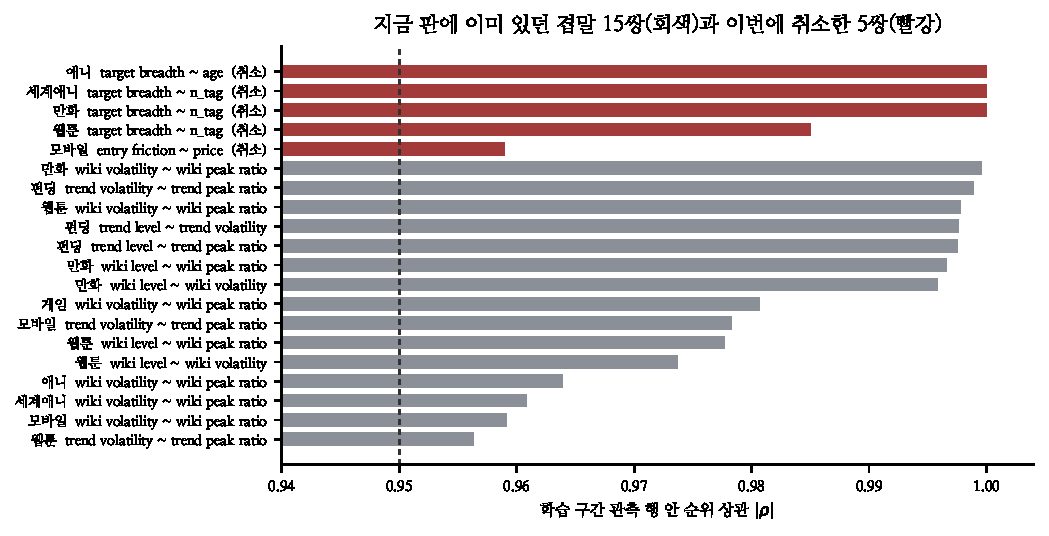
\includegraphics[width=\columnwidth]{figs/dupmap.pdf}
\caption{도메인 안 순위 상관 $|\rho| \ge 0.95$ 인 축 쌍. 빨강 다섯이 이번에
취소한 것이고, 회색 열다섯은 \textbf{취소 전부터 판에 있던} 것이다.}
\end{figure}

라벨을 안 보고 축들끼리의 순위 상관만 보는 가드를 붙였다. 이것은
\textbf{거부권이 아니라 이름표}다 --- 겹치는 축을 막지 않고 ``이것은 새
자료가 아니라 가중 변경''이라고 적는다.

가드를 지금 판에 돌리니 취소한 다섯 말고도 \textbf{이미 15쌍}이 나왔다. 전부
같은 모양이다 --- 검색 · 위키 시계열의 \texttt{level} · \texttt{volatility} ·
\texttt{peak\_ratio} 가 한 방향을 세 번 쓰고 있다(만화
\texttt{wiki\_volatility}\textasciitilde\texttt{wiki\_peak\_ratio} 는
$\rho{=}1.000$). \textbf{판은 오래전부터 그 방향을 세 겹으로 실어 왔다.}

\section{취소한다}

\texttt{lab/recaxes.SPEC} 을 비웠다. 판은 노트 239가 보고한 0.4584에서
\textbf{0.4546으로 내린다.} 노트 213 때와 같은 종류의 후퇴다 --- 점수가 내려간
것이 아니라 점수가 옳아진 것이다. 다만 그때는 자료가 틀렸고 이번에는
\textbf{내 해석이 틀렸다.}

\paragraph{남은 것}
\begin{center}\small
\begin{tabular}{ll}
\hline
갈래 & 왜 \\
\hline
축별 벌점 & 겹말이 흉내 낸 진짜 지렛대다. 안쪽에서 골라야 한다 \\
겹말 15쌍 & 시계열 세 축을 하나로 줄이면 판이 어떻게 되나 \\
$\tau$ 칼날 & 잡음 열 하나로 꺼진다(6 중 3). \texttt{STABLE\_MIN} 이 딱 경계 \\
공유 계수 & 한 도메인 축이 남의 계수를 빼앗는 것을 막는 길 \\
\hline
\end{tabular}
\end{center}

\paragraph{규약} 새 축을 채택하기 전에 \textbf{기존 축과의 도메인 안 순위
상관을 먼저 잰다.} 학습 상관과 시간 조각 부호 일치는 겹말을 못 걸러낸다 ---
겹말은 그 둘을 언제나 통과한다.

\end{document}
